\documentclass[12pt]{article}

\usepackage[margin=1in]{geometry}
\usepackage{setspace}
\usepackage{amsmath, amssymb, amsthm}
\usepackage{hyperref}
\usepackage{tikz}
\usetikzlibrary{arrows.meta}



\doublespacing

\theoremstyle{definition}
\newtheorem{definition}{Definition}
\newtheorem{theorem}{Theorem}
\newtheorem{example}{Example}



\title{From Aristotle to Anti-Foundation}
\author{Mengxiang Jiang\\
Math 629: History of Mathematics}
\date{\today}

\begin{document}

\maketitle

\section{Introduction}

The history of formal logic spans more than two millennia, from Aristotle's codification of the syllogism to Russell's paradox and the resulting foundational crisis in mathematics. This paper traces that arc selectively: Aristotle establishes the enterprise, Leibniz dreams of a universal calculus, Boole begins to realize it for classes, Cantor creates set theory on informal foundations, and Bertrand Russell brings the edifice to a crisis.\footnote{This is nowhere close to a complete history of logic, and the author regrets having no room to discuss many important developments: G\"{o}del's 1931 incompleteness theorems, which showed that no consistent formal system strong enough to express arithmetic can prove all arithmetic truths \cite{godel_1931}; Kripke's possible-worlds semantics for modal logic, developed in the early 1960s, which gave rigorous meaning to operators like $\square$ (necessity) and $\lozenge$ (possibility) by interpreting them over frames of accessible worlds \cite{kripke_completeness}; Gentzen's proof theory and natural deduction \cite{gentzen_1935}; Paul Cohen's 1963 proof, via the method of forcing, that the continuum hypothesis is independent of ZFC (complementing G\"{o}del's earlier consistency result and earning Cohen the 1966 Fields Medal) \cite{cohen_1963}; and, closer to the subject of this paper, a correction to the formula $\square(\square P \rightarrow P) \rightarrow P$ printed on the back of the \href{https://github.com/lucianchauvin/Texas-A-M-Mathematics-Shirt}{Texas A\&M Mathematics Shirt}: the correct statement of L\"{o}b's theorem places $\square P$, not $P$, in the consequent \cite{lob_1955}.} The central argument, however, is not merely historical. The textbook for our class, Victor Katz's \emph{A History of Mathematics}, makes a mathematical claim that is, at minimum, seriously misleading. Katz writes that Russell and Zermelo ``determined that defining sets that contain themselves as elements would lead to contradictions'' \cite{katz}. This is not what Russell's paradox shows. The theory of non-wellfounded sets, developed rigorously by Peter Aczel in the 1980s, demonstrates that sets which contain themselves are perfectly consistent; the contradiction Russell exposed was more specific and more subtle. Understanding the distinction requires engaging with both the history and the mathematics.

\section{Aristotle and the Syllogism}

Logic as a systematic discipline begins with Aristotle (384--322 \textsc{bc}) and his \emph{Organon}, a compilation of six treatises on logic. In the \emph{Prior Analytics}, the third book of the \emph{Organon}, he defines the syllogism: ``A deduction is a discourse in which, certain things being stated, something other than what is stated follows of necessity from their being so'' \cite{aristotle_prior}. What Aristotle accomplished was the extraction of \emph{form} from \emph{content}: the validity of an argument depends not on what the terms refer to but on how they are arranged. In the \emph{Metaphysics} he also articulated the law of non-contradiction: it is impossible for the same attribute both to belong and not to belong to the same subject at the same time \cite{aristotle_metaphysics}. This principle would later be invoked by Russell as the reason his paradox is damaging. Aristotle's logic operated on natural-language predicates rather than formal symbols; the transition to symbolic manipulation required another two thousand years.


\section{Leibniz and the Calculus Ratiocinator}

Gottfried Wilhelm Leibniz (1646--1716) envisioned a complete algebraization of reasoning. In a manuscript of 1679, he wrote of a \emph{characteristica universalis}, a symbolic language in which all concepts would be assigned numerical codes and logical relations between concepts would reduce to arithmetical relations between their codes \cite{leibniz_logical}. Associated with this was the \emph{calculus ratiocinator}: a mechanical procedure for settling disputes by calculation, so that ``two philosophers, when there is a dispute between them, will no more need to fight than two accountants need do: it will suffice for them to take their pens and say to each other, \emph{let us calculate}'' \cite{leibniz_logical}.

Leibniz made partial technical progress, sketching in ``Generales Inquisitiones de Analysi Notionum et Veritatum'' (1686) a system in which propositions are assigned prime-factor encodings and entailment corresponds to divisibility \cite{leibniz_logical}. The project ultimately failed (Leibniz underestimated the complexity of mathematical truth) but it set the agenda for the nineteenth century. Boole, De Morgan, and ultimately Frege all worked in the shadow of Leibniz's dream.

\section{Boole and the Algebra of Classes}

George Boole (1815--1864) was the first to deliver concretely on Leibniz's program. In \emph{An Investigation of the Laws of Thought} (1854), Boole showed that logical operations on classes could be executed as algebraic computation \cite{boole_laws}. He assigned a symbol to each class: if $x$ denotes the class of objects with property $P$ and $y$ those with property $Q$, then $xy$ denotes their intersection, $x + y$ their union (restricted to disjoint classes), and $1 - x$ the complement of $x$ within the universe of discourse~$1$. The law of non-contradiction takes the form $x(1-x) = 0$, which simplifies to $x^2 = x$: applying a class operation twice yields the same result as applying it once.

What Boole made explicit is that the natural objects of logic are \emph{extensions of predicates}: the class $\{x : \phi(x)\}$ of all things satisfying a predicate $\phi$. Logic ceased to be about relationships among named terms and became about algebraic operations on classes. Augustus De Morgan, working in parallel, extended this apparatus to the logic of relations. Together, they demonstrated that Leibniz's \emph{calculus ratiocinator} was achievable in limited domains. The next step, treating these classes not merely as logical abstractions but as mathematical objects with their own arithmetic of size, was Cantor's contribution.

\section{Cantor and Naive Set Theory}

Georg Cantor (1845--1918) created the theory of sets as a mathematical discipline. In 1874, he proved that the real numbers cannot be enumerated: no one-to-one correspondence exists between the natural numbers and the reals \cite{cantor_1874}. The proof forced a distinction between infinite sizes that classical mathematics had not needed to make, and it did so by treating infinite collections as completed wholes comparable by cardinality.

In \emph{Grundlagen einer allgemeinen Mannigfaltigkeitslehre} (1883), Cantor gave an explicit foundational statement: a set (\emph{Menge}) is ``any collection into a whole of definite, well-distinguished objects of our perception or thought'' \cite{cantor_grundlagen}. On this formulation, any coherent property determines a set, the comprehension principle in informal dress. By 1891, his diagonal argument showed that for any set $A$, the power set $\mathcal{P}(A)$ is strictly larger than $A$. Applied to a supposed set of all sets $U$, this gives $|\mathcal{P}(U)| > |U|$, while $\mathcal{P}(U) \subseteq U$ forces $|\mathcal{P}(U)| \leq |U|$, a contradiction. Cantor communicated this and the related paradox of the largest ordinal to Dedekind in 1899 \cite{cantor_letter_dedekind}, but published no formal resolution \cite{ferreiros_labyrinth}.

The instability Cantor left unresolved is precisely the instability Russell exploited. Under Cantor's comprehension principle, the predicate ``does not contain itself'' determines a set, and asking whether that set contains itself produces the contradiction. Russell's paradox is the simplest, most explicit instance of a problem already latent in Cantor's informal foundations. What made it a crisis was that Frege had tried to formalize those foundations, and in doing so had made the problem inescapable.

\section{Russell's Paradox}

\subsection{Frege and the Fatal Letter}

Gottlob Frege's \emph{Grundgesetze der Arithmetik} (1893, 1903) aimed to derive all of arithmetic from pure logic, completing the program that Leibniz had dreamed of and that Cantor's set-theoretic practice had made seem within reach. Frege's \emph{Begriffsschrift} (1879) was explicitly presented as a realization of the \emph{characteristica universalis}. Its central axiom, Basic Law V, states that the extension of the concept $F$ equals the extension of the concept $G$ if and only if $F$ and $G$ apply to exactly the same objects:
\[
\hat{\varepsilon}F(\varepsilon) = \hat{\varepsilon}G(\varepsilon) \iff \forall x\,(Fx \leftrightarrow Gx).
\]
In modern notation, this says that sets are identical when they have the same members; unrestricted comprehension: every predicate defines a set.

On June 16, 1902, Bertrand Russell wrote to Frege identifying a contradiction. Consider the concept ``is a set that does not contain itself.'' By Basic Law V, this concept has an extension; call it $R$. Then:
\[
R \in R \iff R \notin R.
\]
This is a contradiction \cite{russell_letter}. Frege, in his reply six days later, acknowledged the severity: ``Your discovery of the contradiction caused me the greatest surprise and, I would almost say, consternation, since it has shaken the basis on which I intended to build arithmetic'' \cite{frege_reply}.

\subsection{What the Paradox Shows}

The critical point, the one Katz's text obscures, is that Russell's paradox does not condemn all self-containing sets. It condemns a specific set defined by a specific predicate. The set $R$ in Russell's construction is defined by the predicate ``does not contain itself.'' The contradiction arises because this predicate, applied to $R$ itself, generates a sentence that is both true and false. The predicate ``contains itself'' is untouched.

More precisely: under unrestricted comprehension, every predicate $\phi$ determines a set $\{x : \phi(x)\}$. Russell's paradox shows that the predicate $\phi(x) \equiv x \notin x$ cannot determine a consistent set in this framework. This implies that unrestricted comprehension must be restricted; it does not imply that self-membership is inherently contradictory.

The response of Zermelo and subsequent set theorists was to replace unrestricted comprehension with the \emph{Axiom Schema of Separation}: given a set $A$ already assumed to exist, the collection $\{x \in A : \phi(x)\}$ is a set. This blocks the paradox because there is no way to form $R = \{x : x \notin x\}$ without an ambient set to separate from. The Foundation Axiom (Regularity) was later added to the Zermelo--Fraenkel system, asserting that every nonempty set $A$ contains an element $m$ with $m \cap A = \emptyset$. This axiom implies that no set is a member of itself, but it is an \emph{additional restriction}, not a consequence of avoiding paradox.

Katz writes: ``Russell, and Ernst Zermelo (1871--1953) two years earlier, determined that defining sets that contain themselves as elements would lead to contradictions'' \cite{katz}. This is doubly wrong. First, Zermelo's 1908 axiomatization was motivated by avoiding the paradox, not by a prior independent discovery of it (the question of priority is disputed, but Zermelo's proof of the paradox circulated only in informal communications, not in print, before 1905 \cite{moore_zermelo}). Second, and more importantly, the mathematical claim is false: sets that contain themselves do \emph{not} necessarily lead to contradictions. The Foundation Axiom forbids them, but it is an independent axiom that can be dropped or replaced.

\section{Aczel's Anti-Foundation Axiom}

\subsection{Aczel's AFA}

In standard ZFC, the Axiom of Foundation asserts $\forall A\,(A \neq \emptyset \to \exists m \in A\,(m \cap A = \emptyset))$, which rules out $x \in x$ and all infinite descending $\in$-chains. This is mathematically convenient but not forced by the paradox: ZFC$^-$ (ZFC minus Foundation) is consistent if ZFC is. Peter Aczel's 1988 monograph \emph{Non-Well-Founded Sets} replaces Foundation with the \textbf{Anti-Foundation Axiom} (AFA) \cite{aczel}. To state it, we need the language of directed graphs.

\begin{definition}[Accessible pointed graph]
A \emph{graph} is a pair $(G, \to)$ where $G$ is a set of nodes and $\to$ is a binary relation on $G$. A \emph{pointed graph} is a graph with a distinguished node $p$, the \emph{point}. It is \emph{accessible} if every node is reachable from $p$ by a path following $\to$.
\end{definition}

\begin{definition}[Decoration]
A \emph{decoration} of a graph $(G, \to)$ is an assignment $d: G \to V$ (where $V$ is the universe of sets) such that for every node $x$,
\[
d(x) = \{d(y) : x \to y\}.
\]
That is, the set assigned to $x$ has as its elements exactly the sets assigned to the children of $x$.
\end{definition}

\begin{definition}[AFA]
Every accessible pointed graph has a \emph{unique} decoration.
\end{definition}

\begin{definition}[Bisimulation]
A \emph{bisimulation} between two graphs $(G_1, \to_1)$ and $(G_2, \to_2)$ is a relation $Z \subseteq G_1 \times G_2$ such that whenever $x \mathrel{Z} y$: (i) for every $x'$ with $x \to_1 x'$ there exists $y'$ with $y \to_2 y'$ and $x' \mathrel{Z} y'$; and (ii) for every $y'$ with $y \to_2 y'$ there exists $x'$ with $x \to_1 x'$ and $x' \mathrel{Z} y'$. Two nodes (or sets) are \emph{bisimilar} if some bisimulation relates them.
\end{definition}

The uniqueness clause is what distinguishes AFA from weaker anti-foundation axioms (which assert existence but not uniqueness). Uniqueness gives a clean extensionality theory: two sets are equal if and only if they are bisimilar.

\subsection{Self-Containing Sets under AFA}

Under AFA, there exists a set $\Omega$ such that $\Omega = \{\Omega\}$, i.e., $\Omega \in \Omega$. It arises as the unique decoration of the graph with one node $p$ and one edge $p \to p$:

\begin{center}
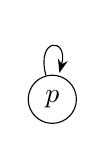
\begin{tikzpicture}[>=Stealth]
  \node[draw, circle] (p) {$p$};
  \path[->] (p) edge [loop above] node {} (p);
\end{tikzpicture}
\end{center}

The decoration must assign to $p$ a set $d(p)$ satisfying $d(p) = \{d(p)\}$. By AFA, such a $d(p)$ exists and is unique. Call it $\Omega$.

\begin{theorem}[Aczel]
The theory \emph{ZFC}$^-$ + \emph{AFA} is consistent relative to \emph{ZFC}. In \emph{ZFC}$^-$ + \emph{AFA}, there exists a unique set $\Omega$ with $\Omega = \{\Omega\}$.
\end{theorem}

The consistency proof proceeds by exhibiting a model: within ZFC, one constructs a universe $V^-$ whose members correspond to certain graph-theoretic structures (Aczel calls them ``hereditarily finite'' systems), and shows this universe satisfies all the axioms of ZFC$^-$ + AFA \cite{aczel}. The key point is that nowhere in this construction does a contradiction appear. The set $\Omega$, with $\Omega \in \Omega$, exists peacefully alongside all the familiar sets.

One might worry that $\Omega \in \Omega$ allows us to reconstruct Russell's paradox, but it does not. Under the Axiom of Separation \cite{zermelo_1908}, we can only form $R_A = \{x \in A : x \notin x\}$ for a given set $A$. Suppose for contradiction that $R_A \in A$. Then $R_A \in R_A \iff R_A \in A \wedge R_A \notin R_A \iff R_A \notin R_A$, a contradiction. So $R_A \notin A$, which is simply the statement that the restricted Russell set falls outside the ambient set $A$, a consistent conclusion with no contradiction. Self-membership is not the culprit. Unrestricted comprehension is.

\section{Katz's Claim}

Katz's error is understandable: in standard ZFC, self-membership is forbidden, so self-containing sets look ``impossible.'' But ``impossible in ZFC'' is not the same as ``leads to contradiction.'' The Axiom of Foundation is an independent axiom adopted for the elegance of the cumulative hierarchy, not because self-membership is inherently inconsistent. What Russell (and independently Zermelo) actually showed is that \emph{unrestricted comprehension} leads to contradiction. Restricting comprehension resolves the paradox; prohibiting self-membership via Foundation is an optional further step that, as AFA demonstrates, can be replaced by its negation without contradiction.

\section{Conclusion}

The line from Aristotle to Russell is a line of increasing formalization: syllogism, algebra of classes, set-theoretic comprehension, Begriffsschrift. Russell's paradox forced a reckoning with what formal systems can and cannot assume. But the lesson of the paradox is not that self-reference is inherently contradictory. It is that mathematical foundations require care. Aczel's Anti-Foundation Axiom shows that a coherent, useful, contradiction-free set theory can accommodate sets like $\Omega = \{\Omega\}$. The history of logic is not the history of discovering all the things we cannot do. It is the history of discovering, with precision, what each choice commits us to.

\bibliographystyle{plain}
\bibliography{references}

\end{document}
